\documentclass[11pt]{amsart}
\pdfsuppressptexinfo=-1
\usepackage[margin=1.1in]{geometry}
\usepackage{amsmath,amssymb,amsthm,mathtools}
\usepackage{booktabs,enumitem,array}
\usepackage{tikz}
\usepackage[hidelinks]{hyperref}

\newtheorem{theorem}{Theorem}[section]
\newtheorem{lemma}[theorem]{Lemma}
\newtheorem{proposition}[theorem]{Proposition}
\newtheorem{corollary}[theorem]{Corollary}
\theoremstyle{definition}
\newtheorem{definition}[theorem]{Definition}
\theoremstyle{remark}
\newtheorem{remark}[theorem]{Remark}
\numberwithin{equation}{section}
\setlength{\emergencystretch}{2em}
\raggedbottom

\newcommand{\file}[1]{\texttt{#1}}
\newcommand{\lean}[1]{\texttt{\detokenize{#1}}}
\newcommand{\LS}{L_{\mathrm S}}
\newcommand{\LM}{L_{\mathrm M}}
\newcommand{\dist}{\operatorname{dist}}
\newcommand{\cl}{\mathrm{cl}}
\newcommand{\ttitle}{The Steiner ratio is at least $0.8564$}
\newcommand{\ptitle}{The Steiner ratio is at least 0.8564}
\newcommand{\rtitle}{The Steiner ratio is at least $0.8564$}
\hypersetup{pdftitle={\ptitle},pdfauthor={Tejasvi Singh Tomar}}
\newcommand{\RHO}{\tfrac{2141}{2500}}
\newcommand{\NREC}{555{,}102{,}905}
\newcommand{\NOK}{427{,}276{,}647}
\newcommand{\NCOMBO}{42{,}303}
\newcommand{\CAPSTAR}{0.856}
\newcommand{\CAPONE}{0.8572}
\newcommand{\SUPPDOI}{10.5281/zenodo.23716011}
\newcommand{\REPOURL}{https://github.com/tejasvi/steiner-ratio-bound/tree/v4}
\newcommand{\NUNITS}{455{,}318}
\newcommand{\KRECS}{1{,}200}
\newcommand{\LEANVERSION}{v4.35.0-rc3}
\newcommand{\MATHLIBCOMMIT}{c55e6e786f49}
\newcommand{\NJOBS}{648{,}325}
\newcommand{\NSHARDS}{482}
\newcommand{\NAX}{496}
\newcommand{\AUDITTEXT}{The repository describes an independent rebuild of this proof and replays of its exported proofs by three kernel checkers.}

\begin{document}

\title[\rtitle]{\ttitle}
\author{Tejasvi Singh Tomar}
\renewcommand{\urladdrname}{{\itshape ORCID}}
\urladdr{\href{https://orcid.org/0000-0003-4668-3639}{https://orcid.org/0000-0003-4668-3639}}
\subjclass[2020]{05C05; 90C27, 65G40, 68V20}
\keywords{Steiner ratio, Gilbert--Pollak conjecture, Steiner minimal tree, minimum spanning tree, computer-assisted proof, interval arithmetic, formal verification, Lean 4}

\begin{abstract}
The Steiner ratio is the infimum, over finite sets of points in the Euclidean plane, of the length of a Steiner minimal tree divided by the length of a minimum spanning tree. Gilbert and Pollak conjectured in 1968 that it equals $\sqrt3/2\approx0.8660$, and the conjecture is open. We prove that it is at least $2141/2500=0.8564$, improving the bound $0.8559$ of Ke, Huang, Shu, He, Gai and Wang. Their method reduces the induction step of Du and Hwang's 1983 proof of the bound $0.8$ to finitely many inequalities on boxes in a space of local configurations of a Steiner minimal tree, which are checked by computer. These inequalities use estimates for the positions of terminals outside the local configuration. We prove all the geometric lemmas that our certificate uses, filling gaps in two proofs of Ke et al., and we add two such estimates that hold for more parameter values than the published ones. Within this method some new estimate is necessary: with the published estimates, no certificate of this kind reaches $\CAPSTAR$, whatever the boxes. The computer-assisted part is also verified in Lean~4, by a proof whose checks all run in Lean's kernel; the rest of the argument enters the formal proof as hypotheses.
\end{abstract}

\maketitle

\section{Introduction}\label{sec:intro}

For a finite set $V$ of points in the Euclidean plane, let $\LS(V)$ be the length of a Steiner minimal tree for $V$, that is, of a shortest network that connects the points of $V$ and may use further vertices, and let $\LM(V)$ be the length of a minimum spanning tree of $V$. The \emph{Steiner ratio} is
\[
\rho_S=\inf\Bigl\{\frac{\LS(V)}{\LM(V)}:V\subset\mathbb R^2,\ 2\le|V|<\infty\Bigr\}.
\]
Gilbert and Pollak conjectured that $\rho_S=\sqrt3/2=0.8660\ldots$, the value for the vertices of an equilateral triangle \cite{GP68}. Lower bounds followed: $\frac12$, attributed to Moore in \cite{GP68}; $1/\sqrt3=0.577\ldots$ by Graham and Hwang in 1976 \cite{GH76}; $0.743$ by Chung and Hwang in 1978 \cite{CH78}; $0.8$ by Du and Hwang in 1983 \cite{DH83}; and $0.824$ by Chung and Graham in 1985 \cite{CG85}. The conjecture is known for sets of at most four points \cite{Pol78,DYH82}, five points \cite{DHY85} and six points \cite{RT91}. Du and Hwang announced a proof of the conjecture \cite{DH90,DH92}; Ivanov and Tuzhilin explained why the argument does not prove it \cite{IT12}. In 2026, Ke, Huang, Shu, He, Gai and Wang gave a computer-assisted proof of $\rho_S\ge0.8559$ \cite{KHSHGW}.

\begin{theorem}\label{thm:main}
For every finite set $V$ of points in the plane, $\LS(V)\ge\RHO\,\LM(V)$. Hence $\rho_S\ge2141/2500=0.8564$.
\end{theorem}

The proof follows the method of \cite{KHSHGW}, which rests on the induction of Du and Hwang \cite{DH83}. To prove $\LS(V)\ge\rho\LM(V)$ for all $V$ and a constant $\rho$, one removes a few edges of a Steiner minimal tree near a leaf, connects the separated terminals to the other terminals by segments, and reconnects the rest of the tree by a new network; the segments, together with a minimum spanning tree of the other terminals, connect all the terminals. If the length removed is at least the length added plus $\rho$ times the length of the connecting segments, that is, if the \emph{cost} of this \emph{splitting} is at most $0$, then the inequality for sets with fewer points gives it for the whole set (Lemma~\ref{lem:dh}). Near a suitable leaf, every full Steiner minimal tree with at least five terminals contains a local configuration of one of two types, which is determined up to similarity by six or eight edge lengths divided by the length of the edge at the leaf (Lemmas~\ref{lem:local} and~\ref{lem:coords}, Figure~\ref{fig:conf}). For each type, \cite{KHSHGW} fixes a finite list of splittings and bounds the cost of each by an explicit function of these parameters. The parameter space is covered by boxes, and each box carries one splitting whose cost bound is at most $0$ at the vertices of the box; this suffices because along every line parallel to a coordinate axis the cost bounds first do not increase and then do not decrease (Lemma~\ref{lem:vertex}). Some splittings connect to a terminal that lies outside the configuration, at the end of a chain of Steiner points. Each configuration has two such \emph{hidden terminals}, $E$ and $F$ (Section~\ref{sec:chains}), and geometric lemmas of \cite{KHSHGW} and \cite{DH83} bound their positions under conditions on the parameters.

We use this method, the splitting tables of \cite{KHSHGW} and a modified version of the generator of boxes of \cite{KHSHGW}. Our proof differs from that of \cite{KHSHGW} in four ways. First, we prove the reduction to the two types of configuration and every bound for the hidden terminals that our certificate uses, relying only on standard facts about Steiner minimal trees and on the known case of the conjecture for at most four points. Our proofs of the published bounds rest on an exchange inequality and a turning-number argument (Lemmas~\ref{lem:exch} and~\ref{lem:trapprinciple}). Two of the proofs in \cite{KHSHGW} have gaps (Remark~\ref{rem:pku}); we give complete proofs of the statements that we use.

Second, we add two bounds. The published bound for $F$ requires $f\le d$, where $d$ and $f$ are the lengths of the edges $YD$ and $ZQ$ (Figure~\ref{fig:conf}), and one of the published bounds for $E$ requires a linear condition on the parameters. These restrictions stop the method of \cite{KHSHGW}: by Proposition~\ref{prop:cap}, no certificate of this form built on the lemmas of \cite{KHSHGW} reaches $\CAPSTAR$, since at the configurations near a configuration $w_*$ with $f$ slightly larger than $d$, every splitting of the form used in \cite{KHSHGW}, not only those in its tables, either requires a bound for $F$ that these lemmas do not give or has a positive cost bound with them. Lemma~\ref{lem:y2} gives the published bound for $F$ in that type also when $f>d$, under an explicit inequality between lengths, and Lemma~\ref{lem:x2} replaces the linear condition for $E$ by a less restrictive condition with the same conclusion. Both apply at $w_*$ with a margin, and hence near it. Their proofs compare the Steiner tree with networks that replace several of its edges at once, not only with networks obtained by exchanging one edge.

Third, when a splitting reconnects four points, we bound the length of the new network by that of an explicit network with two Steiner points, instead of the closed formula of \cite{KHSHGW} for the length of a full Steiner tree, which is an upper bound only where such a tree exists, so that \cite{KHSHGW} imposes conditions for its existence. Fourth, our certificate consists of $\NREC$ boxes. A checker that shares no code with the generator verifies, in ball arithmetic, the inequality of every box that meets the domain of its family, and a second program verifies that the boxes of each family tile the orthant $[0,\infty)^n$ of its coordinates.

The conditional bound $0.860$ of \cite{S26}, listed in Tao's repository of optimization constants \cite{Tao}, uses the generator and the lemmas of \cite{KHSHGW}; Remark~\ref{rem:S26} explains how Proposition~\ref{prop:cap} bears on it.

We have also verified the computer-assisted part in the Lean~4 proof assistant \cite{Lean4} with the Mathlib library \cite{Mathlib}. A checking program written in Lean verifies the boxes of all four families, including the covering of the domains, and a Lean proof shows that whenever the program accepts, the inequalities of Section~\ref{sec:ver} hold on the whole domain of each family. From this, Lean derives Theorem~\ref{thm:main}, with $\LS$ and $\LM$ defined in Lean, under hypotheses that state the rest of the argument. In one formal proof the checks are run as compiled code; a second proof of the same statement checks the same boxes with a program in integer arithmetic whose runs are evaluated by Lean's kernel, so that it relies on the kernel instead of code generated by Lean's compiler.

Section~\ref{sec:red} sets up the induction and the two types of configuration, and Section~\ref{sec:trap} proves the bounds for the hidden terminals. Sections~\ref{sec:ver} and~\ref{sec:cert} describe the functions checked on the boxes and the certificate, and complete the proof of Theorem~\ref{thm:main}. Section~\ref{sec:cap} proves Proposition~\ref{prop:cap}, and Section~\ref{sec:lean} states the formal theorems and their hypotheses, and Appendix~\ref{app:lean} describes the checking programs of the formal proofs.

\section{Splittings and local configurations}\label{sec:red}

\subsection{Steiner minimal trees}
We use the following facts \cite{GP68}. Every finite set $V$ with $|V|\ge2$ has a Steiner minimal tree (SMT). It is a tree whose vertices are the points of $V$, called \emph{terminals}, and possibly further points, called \emph{Steiner points}; its edges are segments, and two edges meet only at a common endpoint. Every Steiner point has degree three, and its three edges make angles of $120^\circ$. There are at most $|V|-2$ Steiner points. An SMT with exactly $|V|-2$ Steiner points is \emph{full}; then every terminal is a leaf. Conversely, if every terminal is a leaf, counting degrees shows that there are $|V|-2$ Steiner points. We call a connected finite union of segments a \emph{network}; no network that contains $V$ is shorter than an SMT for $V$.

\subsection{Splittings}
For a tree $S$ and a set $S^-$ of its edges, $S\setminus S^-$ denotes the union of the edges of $S$ that are not in $S^-$. For a finite set $N$ of segments, $L(N)$ is the sum of their lengths; a network formed by these segments has length at most $L(N)$.

\begin{definition}\label{def:split}
Let $S$ be an SMT for $V$. A \emph{splitting} of $S$ is a tuple $(V^*,S^-,S^+,t^*)$ such that
\begin{enumerate}[label=(\alph*)]
\item $V^*$ is a nonempty proper subset of $V$;
\item $S^-$ is a set of edges of $S$;
\item $S^+$ is a finite set of segments such that $V\setminus V^*$ lies in one connected component of $(S\setminus S^-)\cup S^+$;
\item $t^*$ is a finite set of segments with endpoints in $V$ such that every point of $V^*$ is joined to a point of $V\setminus V^*$ by a path in $t^*$.
\end{enumerate}
Its \emph{cost} at $\rho$ is $\rho L(t^*)+L(S^+)-L(S^-)$.
\end{definition}

This is weaker than \cite[Definition~13]{KHSHGW}, which also asks that no point of $V^*$ is incident to $S\setminus S^-$, that $(S\setminus S^-)\cup S^+$ is a Steiner tree, and that no path in $t^*$ joins two points of $V\setminus V^*$; Lemma~\ref{lem:dh} holds without these conditions. The following lemma is stated in \cite[Lemma~14]{KHSHGW}, where it is attributed to \cite[Lemma~3]{DH83}. We include a proof for the weaker definition.

\begin{lemma}\label{lem:dh}
Let $\rho>0$ and $n\ge2$, and suppose that $\LS(W)\ge\rho\LM(W)$ for every set $W$ with $2\le|W|<n$. Let $S$ be an SMT for a set $V$ of $n$ points. If $S$ has a splitting of cost at most $0$ at $\rho$, then $\LS(V)\ge\rho\LM(V)$.
\end{lemma}

\begin{proof}
Let $(V^*,S^-,S^+,t^*)$ be the splitting and $V'=V\setminus V^*$, so $1\le|V'|<n$. By (c), a connected component of $(S\setminus S^-)\cup S^+$ is a network containing $V'$; hence $\LS(V')\le L(S)-L(S^-)+L(S^+)$. If $|V'|\ge2$, the hypothesis gives $\rho\LM(V')\le\LS(V')$; if $|V'|=1$, both sides are $0$. The edges of a minimum spanning tree of $V'$ together with the segments of $t^*$ form a connected graph on $V$ by (d), whose edges are segments between points of $V$; so $\LM(V)\le\LM(V')+L(t^*)$. Hence
\[
\rho\LM(V)\le\LS(V')+\rho L(t^*)\le L(S)-\bigl(L(S^-)-L(S^+)-\rho L(t^*)\bigr)\le L(S)=\LS(V).\qedhere
\]
\end{proof}

\subsection{Reduction to full trees}

\begin{lemma}\label{lem:nonfull}
Let $\rho>0$ and $n\ge3$, and suppose that $\LS(W)\ge\rho\LM(W)$ for every set $W$ with $2\le|W|<n$. If a set $V$ of $n$ points has an SMT $S$ in which some terminal has degree at least two, then $\LS(V)\ge\rho\LM(V)$.
\end{lemma}

\begin{proof}
Let $x$ be such a terminal, let $S_1,\dots,S_k$ ($k\ge2$) be the closures of the components of $S\setminus\{x\}$, and let $V_i=V\cap S_i$. Each $S_i$ contains $x$ and a leaf of $S$, which is a terminal, so $|V_i|\ge2$; and $V_i$ misses the leaves of $S$ in the other branches; hence $|V_i|<n$. Each $S_i$ is an SMT for $V_i$, since a shorter network for $V_i$ could replace it. The minimum spanning trees of the $V_i$ all contain $x$, so their union is a connected graph on $V$, and $\LM(V)\le\sum_i\LM(V_i)\le\sum_iL(S_i)/\rho=\LS(V)/\rho$.
\end{proof}

\subsection{Local configurations}

\begin{lemma}\label{lem:local}
Let $S$ be a full SMT for a set of $n\ge5$ terminals. Then $S$ has Steiner points $X$, $Y$, $Z$ and terminals $A$, $B$ such that the neighbours of $X$ are $A$, $B$, $Y$; the neighbours of $Y$ are $X$, $Z$ and a vertex $D$ that is either a terminal or a Steiner point whose two other neighbours $U$, $V$ are terminals; and $Z$ has two neighbours $R$, $Q$ besides $Y$. If $n=5$, then $D$, $R$ and $Q$ are terminals.
\end{lemma}

\begin{proof}
The Steiner points span a subtree with $n-2\ge3$ vertices, which contains a path with two edges. A longest path in this subtree ends at two of its leaves, each of which is adjacent to two terminals; so $S$ has a path between two leaves with at least four edges. Let $v_0,v_1,\dots,v_k$ be a longest such path, so $k\ge4$, and put $A=v_0$, $X=v_1$, $Y=v_2$, $Z=v_3$. The third neighbour $B$ of $X$ is a terminal: otherwise it would have a further neighbour, and a path from a leaf behind $B$ through $B,X,Y,\dots,v_k$ would have at least $k+1$ edges. Let $D$ be the third neighbour of $Y$. If a neighbour of $D$ other than $Y$ were a Steiner point, a leaf behind it would give a path with at least $k+1$ edges ending at $v_k$; so $D$ is a terminal or a Steiner point whose other two neighbours are terminals. Since $k\ge4$, $Z=v_3$ is not an end of the path and is therefore a Steiner point; let $R$, $Q$ be its other neighbours. If $n=5$, the only Steiner points are $X$, $Y$, $Z$, so $D$, $R$, $Q$ are terminals.
\end{proof}

Following \cite{KHSHGW}, we call the configuration \emph{d\_regular} if $D$ is a terminal and \emph{d\_steiner} otherwise. We write $T_R$ and $T_Q$ for the closures of the components of $S\setminus[Z,R]$ and $S\setminus[Z,Q]$ that contain $R$ and $Q$; every terminal other than $A$, $B$ and $D$ (or $U$, $V$) lies in $T_R\cup T_Q$.

We identify the plane with $\mathbb C$ and put $\omega=e^{i\pi/3}$, so that $\omega$ and $\bar\omega$ are the unit vectors at angles $60^\circ$ and $-60^\circ$.

\begin{lemma}\label{lem:coords}
In Lemma~\ref{lem:local}, after possibly exchanging the names $A,B$, the names $R,Q$ and the names $U,V$, and after a similarity of the plane, possibly reversing orientation, we have
\begin{equation}\label{eq:coords}
\begin{gathered}
A=0,\quad X=1,\quad B=1+b\omega,\quad Y=1+s\bar\omega,\quad D=Y+d,\quad Z=Y-c\omega,\\
R=Z-e,\quad Q=Z+f\bar\omega,\qquad\text{and in d\_steiner}\quad U=D+u\omega,\quad V=D+v\bar\omega,
\end{gathered}
\end{equation}
with positive numbers $b,s,c,d,e,f$ (and $u,v$), the lengths of the edges $XB$, $XY$, $YZ$, $YD$, $ZR$, $ZQ$ (and $DU$, $DV$) divided by $|AX|$. In d\_steiner one may moreover assume that $\max(u,v)\le\max(b,1)$.
\end{lemma}

\begin{proof}
Traversing $X\to Y$, one of the edges $YD$, $YZ$ turns left by $60^\circ$ and the other turns right. Reflecting the plane if necessary, $YD$ turns left. Exactly one of the two leaves at $X$ is such that $A\to X\to Y$ turns right; we call it $A$ and the other one $B$, which is allowed since both are terminals adjacent to $X$. A translation, a rotation and a scaling by $1/|AX|$ give $A=0$ and $X=1$. Since the edges at each Steiner point make angles of $120^\circ$, the edge $XY$ has direction $-60^\circ$ and $XB$ direction $60^\circ$; $YD$ has direction $0^\circ$ and $YZ$ direction $-120^\circ$. At $Z$ we call $R$ the neighbour in direction $180^\circ$ and $Q$ the one in direction $-60^\circ$, and in d\_steiner we call $U$ and $V$ the neighbours of $D$ in directions $60^\circ$ and $-60^\circ$. This gives \eqref{eq:coords}.

In d\_steiner, suppose $\max(u,v)>\max(b,1)$. The vertex $D$ with its leaves $U$, $V$ and the vertex $X$ with its leaves $A$, $B$ are both attached to $Y$; thus exchanging their roles gives another labelling that satisfies Lemma~\ref{lem:local} with $D$ a Steiner point. After normalizing it as above, the new unit length is $|DU|$ or $|DV|$, the new $\max(b,1)$ is the old $\max(u,v)$ divided by it, and the new $\max(u,v)$ is the old $\max(b,1)$ divided by it. Hence the new parameters satisfy $\max(u,v)<\max(b,1)$.
\end{proof}

\begin{figure}[ht]
\centering
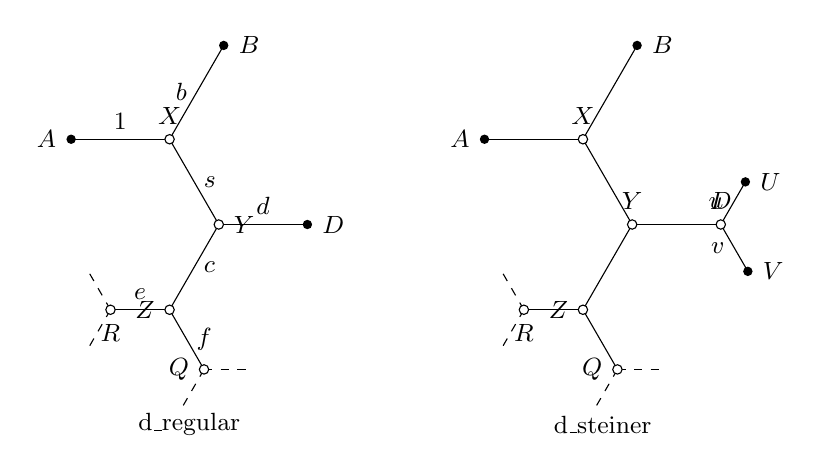
\begin{tikzpicture}[scale=1.25,every node/.style={font=\small},dot/.style={circle,fill,inner sep=1.2pt},sp/.style={circle,draw,fill=white,inner sep=1.2pt}]
\begin{scope}
\coordinate (A) at (0,0); \coordinate (X) at (1,0); \coordinate (B) at (1.550,0.953);
\coordinate (Y) at (1.500,-0.866); \coordinate (D) at (2.400,-0.866); \coordinate (Z) at (1.000,-1.732);
\coordinate (R) at (0.400,-1.732); \coordinate (Q) at (1.350,-2.338);
\draw (A)--(X) node[midway,above]{$1$}; \draw (X)--(B) node[midway,left]{$b$}; \draw (X)--(Y) node[midway,right]{$s$};
\draw (Y)--(D) node[midway,above]{$d$}; \draw (Y)--(Z) node[midway,right]{$c$}; \draw (Z)--(R) node[midway,above]{$e$};
\draw (Z)--(Q) node[midway,right]{$f$};
\draw[dashed] (R)--++(-0.25,0.433); \draw[dashed] (R)--++(-0.25,-0.433);
\draw[dashed] (Q)--++(0.5,0); \draw[dashed] (Q)--++(-0.25,-0.433);
\node[dot,label=left:$A$] at (A) {}; \node[sp,label=above:$X$] at (X) {}; \node[dot,label=right:$B$] at (B) {};
\node[sp,label=right:$Y$] at (Y) {}; \node[dot,label=right:$D$] at (D) {}; \node[sp,label=left:$Z$] at (Z) {};
\node[sp,label=below:$R$] at (R) {}; \node[sp,label=left:$Q$] at (Q) {};
\node at (1.2,-2.9) {d\_regular};
\end{scope}
\begin{scope}[xshift=4.2cm]
\coordinate (A) at (0,0); \coordinate (X) at (1,0); \coordinate (B) at (1.550,0.953);
\coordinate (Y) at (1.500,-0.866); \coordinate (D) at (2.400,-0.866); \coordinate (Z) at (1.000,-1.732);
\coordinate (R) at (0.400,-1.732); \coordinate (Q) at (1.350,-2.338); \coordinate (U) at (2.650,-0.433); \coordinate (V) at (2.675,-1.342);
\draw (A)--(X); \draw (X)--(B); \draw (X)--(Y); \draw (Y)--(D); \draw (Y)--(Z); \draw (Z)--(R); \draw (Z)--(Q);
\draw (D)--(U) node[midway,left]{$u$}; \draw (D)--(V) node[midway,left]{$v$};
\draw[dashed] (R)--++(-0.25,0.433); \draw[dashed] (R)--++(-0.25,-0.433);
\draw[dashed] (Q)--++(0.5,0); \draw[dashed] (Q)--++(-0.25,-0.433);
\node[dot,label=left:$A$] at (A) {}; \node[sp,label=above:$X$] at (X) {}; \node[dot,label=right:$B$] at (B) {};
\node[sp,label=above:$Y$] at (Y) {}; \node[sp,label=above:$D$] at (D) {}; \node[sp,label=left:$Z$] at (Z) {};
\node[sp,label=below:$R$] at (R) {}; \node[sp,label=left:$Q$] at (Q) {};
\node[dot,label=right:$U$] at (U) {}; \node[dot,label=right:$V$] at (V) {};
\node at (1.2,-2.9) {d\_steiner};
\end{scope}
\end{tikzpicture}
\caption{The two local configurations of Lemma~\ref{lem:local} in the coordinates~\eqref{eq:coords}. Filled dots are terminals, open dots are Steiner points or, at $R$ and $Q$, vertices that may be of either kind; the dashed edges continue into $T_R$ and $T_Q$.}\label{fig:conf}
\end{figure}

\subsection{The subcases}
Every configuration has $f\le d$ or $f\ge d$. The certificate treats four families: d\_regular with $f\le d$ and with $f\ge d$, and d\_steiner with $f\le d$ and with $f\ge d$. In the parameter space of a family, the coordinates are $(b,c,d,s,e,f)$ for d\_regular and $(b,c,d,s,u,v,e,f)$ for d\_steiner; for d\_steiner with $f\ge d$ we use $(b,c,d,s,u,v,e)$ and the value $f=d$, see Lemma~\ref{lem:ext}.

\subsection{Small sets}\label{sec:small}
For $|V|=2$ the ratio is $1$. For three points with sides $a\le b'\le c'$, let $\gamma$ be the angle opposite $c'$, so $\gamma\ge60^\circ$ and $\LM=a+b'$. If $\gamma\ge120^\circ$, the SMT is the minimum spanning tree. Otherwise
\[
\LS^2=\tfrac12\bigl(a^2+b'^2+c'^2\bigr)+2\sqrt3\,\mathrm{area}=a^2+b'^2+2ab'\sin(\gamma-30^\circ)\ge a^2+ab'+b'^2\ge\tfrac34(a+b')^2.
\]
For four points the conjecture was proved by Pollak \cite{Pol78}; a shorter proof is in \cite{DYH82}. Thus $\LS(V)\ge\frac{\sqrt3}2\LM(V)>\RHO\LM(V)$ whenever $2\le|V|\le4$.

\section{Hidden terminals}\label{sec:trap}

Throughout this section $S$ is a full SMT in the position of Lemma~\ref{lem:coords}, with at least five terminals. For a point $p$ and a segment $\sigma$, $\dist(p,\sigma)$ is the distance between them, and $B(p,r)$ is the open disk of radius $r$ about $p$.

\subsection{Chains}\label{sec:chains}
Put $A_0=A$, $A_1=X$, $A_2=Y$, $A_3=Z$, $A_4=R$. If $A_k$ ($k\ge4$) is a Steiner point, let $A_{k+1}$ be its neighbour reached by turning right by $60^\circ$. The walk never goes back; hence it follows a path of the tree and ends at a leaf $A_N$, $N\ge4$, which is a terminal; we call it $E$. We write $\sigma_k=[A_{k-1},A_k]$ and $a_k=|\sigma_k|$, so $a_1=1$, $a_2=s$, $a_3=c$, $a_4=e$, and $\sigma_k$ has direction $\bar\omega^{\,k-1}$. Similarly the walk $D\to Y\to Z\to Q$ turns left by $60^\circ$ at $Y$ and at $Z$; continued by left turns at Steiner points, it ends at a terminal $F$. In d\_steiner the walk $V\to D\to Y\to Z\to Q\to\cdots$ also turns left at every vertex and ends at the same $F$.

The terminal $E$ lies in $T_R$ and $F$ lies in $T_Q$. These two trees are disjoint and contain none of $A$, $B$, $D$, $U$, $V$. In particular $E\ne F$, and both are terminals of $V\setminus\{A,B,D,U,V\}$.

\subsection{Exchange and trapping}

\begin{lemma}\label{lem:exch}
Let $p,q$ be points of $S$ and let $\tau$ be a segment contained in an edge of $S$ and in the path of $S$ from $p$ to $q$. Then $|pq|\ge|\tau|$. In particular, for $0\le u\le k-2$,
\begin{equation}\label{eq:E1}
\dist(A_u,\sigma_k)\ge\max(a_{u+1},\dots,a_{k-1}),
\end{equation}
and $|A_uA_v|\ge a_t$ for $u<t\le v$.
\end{lemma}

\begin{proof}
Removing the relative interior of $\tau$ splits $S$ into two parts, one containing $p$ and the other $q$; no terminal is removed. Adding $[p,q]$ gives a network that contains all terminals and has length $L(S)-|\tau|+|pq|$, which is at least $L(S)$. For \eqref{eq:E1}, the path from $A_u$ to a point of $\sigma_k$ contains $\sigma_{u+1},\dots,\sigma_{k-1}$.
\end{proof}

A point $p$ is to the \emph{right} of an oriented line $\ell$ through $p_0$ with unit direction $\delta$ if $\operatorname{Im}((p-p_0)\bar\delta)<0$. Below, $\lambda_\ell(p)=\operatorname{Im}((p-p_0)\bar\delta)$ is the signed distance to the left of $\ell$.

\begin{lemma}[trap principle]\label{lem:trapprinciple}
Let $1\le m\le N$, and let $\ell$ be the line through $A_{m-1}$ and $A_m$, oriented by $\sigma_m$. Let $P$ be a simple polygon in the closed half-plane to the right of $\ell$ whose boundary consists of pieces of the edges $\sigma_1,\dots,\sigma_m$, a segment $J=[A_m,z_0]\subset\ell$ with $z_0$ beyond $A_m$, and further segments called doors, such that $A_m$ lies in the relative interior of the side of $P$ that contains $J$. If no point of the tail $A_mA_{m+1}\cdots A_N$ other than $A_m$ lies on a door outside $J$, then the tail lies in $P$; hence $E\in P$.
\end{lemma}

\begin{proof}
If $m=N$, then $E=A_m\in P$. Let $m<N$. Near $A_m$ the polygon coincides with the half-disk to the right of $\ell$, and $\sigma_{m+1}$ turns right by $60^\circ$, so the tail enters the interior of $P$. Suppose it leaves $P$, and let $z$ be the first point of the tail after $A_m$ that lies on $\partial P$. The tail meets the edges $\sigma_1,\dots,\sigma_m$ only at $A_m$, since $S$ is a tree whose edges meet only at common endpoints, and it does not meet a door outside $J$; so $z\in J\setminus\{A_m\}$. The tail from $A_m$ to $z$ followed by $[z,A_m]$ is a simple closed polygon in the closed right half-plane of $\ell$. Its angle at $A_m$ is $60^\circ$; thus it is traversed counterclockwise and its turning angles add up to $360^\circ$. They are $120^\circ$ at $A_m$, $-60^\circ$ at each vertex of the tail before $z$, and $180^\circ-\varphi$ at $z$ for some $\varphi\in(0^\circ,180^\circ)$, since the edge that arrives at $z$ does not lie on $\ell$ (its earlier points would lie on $\partial P$). Their sum is less than $300^\circ$, a contradiction.
\end{proof}

\begin{lemma}\label{lem:T}
Let $0\le u<t\le v<N$, let $\ell$ be the line through $A_v$ and $A_{v+1}$, oriented by $\sigma_{v+1}$, and let $H$ be the foot of the perpendicular from $A_u$ to $\ell$. Suppose that
\begin{enumerate}[label=\textup{(T\arabic*)}]
\item $H$ lies on the ray from $A_v$ through $A_{v+1}$;
\item $|A_uH|<a_t$;
\item $A_u,\dots,A_v$ lie in the closed half-plane to the right of $\ell$, and $A_{u+1},\dots,A_{v-1}$ in the open one;
\item $[A_u,H]$ meets the edges $\sigma_{u+1},\dots,\sigma_t$ only at $A_u$.
\end{enumerate}
Then $H$ lies beyond $A_{v+1}$, the polygon $P=A_uA_{u+1}\cdots A_vH$ is simple, and $E\in P$.
\end{lemma}

Lemma~\ref{lem:T} is a form of \cite[Lemma~8]{KHSHGW} with the additional hypotheses (T3) and (T4); see Remark~\ref{rem:pku}.

\begin{proof}
The door $[A_u,H]$ lies in $B(A_u,a_t)$ by (T2), and by \eqref{eq:E1} the edges $\sigma_k$ with $k\ge t+1$ avoid this disk. In particular $H\notin\sigma_{v+1}$, so by (T1) $H$ lies beyond $A_{v+1}$. By (T3) the edges $\sigma_{u+1},\dots,\sigma_v$ meet $\ell$ only at $A_v$, and at $A_u$ if $A_u\in\ell$, in which case $H=A_u$. The door is perpendicular to $\ell$; hence it meets $[A_v,H]$ only at $H$; by (T4) and the disk it meets $\sigma_{u+1},\dots,\sigma_v$ only at $A_u$. Therefore $P$ is simple, and it lies in the closed right half-plane of $\ell$. Lemma~\ref{lem:trapprinciple} with $m=v+1$, $J=[A_{v+1},H]$ and the door $[H,A_u]$ applies, since the tail consists of edges $\sigma_k$ with $k\ge v+2\ge t+2$.
\end{proof}

\subsection{\texorpdfstring{Bounds for $E$ from the published lemmas}{Bounds for E from the published lemmas}}
The following lemmas are Lemmas~27, 29, 30, 33 and~36 of \cite{KHSHGW}; the first is due to Du and Hwang \cite[Lemma~2]{DH83}. Let $\ell_5$ be the line through $A_4=R$ in direction $\omega^2=e^{2\pi i/3}$, which contains $\sigma_5$ if $N\ge5$, and let $W=1-c-e$ be its intersection with the real axis; then $|RW|=s+c$. The pentagon $\Pi=WA_1A_2A_3A_4$ is convex, it is traversed clockwise, and it lies to the right of $\ell_5$ oriented by $\omega^2$.

\begin{lemma}[{\cite[Lemma~2]{DH83}, \cite[Lemma~27]{KHSHGW}}]\label{lem:L0}
If $c\le1$, then $E\in\Pi$ and $|AE|\le\max(|AY|,|AZ|)$.
\end{lemma}

\begin{proof}
If $N=4$, then $E=R$. Let $N\ge5$. We first show $a_5<s+c$, that is, $A_5$ lies strictly between $R$ and $W$. If $c+e\le1$, then $W\in\sigma_1$, and $a_5\ge s+c$ would put $W$ on $\sigma_5$, while $\dist(\sigma_1,\sigma_5)\ge a_2>0$ by Lemma~\ref{lem:exch}. If $c+e>1$ and $c<1$, then $|AW|=c+e-1<e=a_4$, so $W\in B(A,a_4)$, which $\sigma_5$ avoids by \eqref{eq:E1}. If $c=1$, the foot of the perpendicular from $A$ to $\ell_5$ is at distance $1+s-e/2$ from $R$, and $0<e\le1+s$ because $|AR|^2-e^2=(1+s)(1+s-e)$ and $|AR|\ge e$ (Lemma~\ref{lem:exch}); so the foot lies on $[R,W]$, at distance $\frac{\sqrt3}2e<e$ from $A$. By \eqref{eq:E1}, $\sigma_5$ does not contain the foot; hence it ends before reaching it, and $a_5<s+c$.

Now apply Lemma~\ref{lem:trapprinciple} with $m=5$, $P=\Pi$ and $J=[A_5,W]$. If $c+e\le1$, the boundary of $\Pi$ consists of $[W,A_1]\subset\sigma_1$, $\sigma_2$, $\sigma_3$, $\sigma_4$ and $[A_4,W]$, and there is no door. If $c+e>1$, the door is $[W,A]$. All its points other than $W$ lie in $B(A,e)$, since $|AW|=c+e-1\le e$, and the tail consists of edges $\sigma_k$ with $k\ge6$, which avoid $B(A,a_4)$ by \eqref{eq:E1}; the point $W$ lies on $J$. Consequently $E\in\Pi$.

For the bound, $|AA_1|=1\le|AA_2|$. Let $x_3=1+(s-c)/2>0$ be the real part of $A_3$. From $|AA_4|^2=|AA_3|^2-e(2x_3-e)$ and $|AA_4|\ge e$ we get $e\le|AA_3|^2/(2x_3)$, and $4x_3^2-|AA_3|^2=3(1+s)(1-c)\ge0$ gives $e\le2x_3$, hence $|AA_4|\le|AA_3|$. Finally $|AW|\le\max(1,e)\le|AA_4|$, because $|AA_4|\ge a_1$ and $|AA_4|\ge a_4$.
\end{proof}

\begin{lemma}[{\cite[Lemmas~29 and~30]{KHSHGW}}]\label{lem:L12}
Suppose that $c+e\ge1$ and that $e<1-c+\frac2{\sqrt3}s$ or $e<1+\bigl(\frac2{\sqrt3}-1\bigr)c$. Let $H$ be the foot of the perpendicular from $A$ to $\ell_5$. Then $E$ lies in the polygon $AA_1A_2A_3A_4H$ and $|AE|\le\max\bigl(1,|AY|,|AZ|,|AR|,\frac{\sqrt3}2(c+e-1)\bigr)$.
\end{lemma}

\begin{proof}
If $N=4$, then $E=R$. Otherwise we apply Lemma~\ref{lem:T} with $(u,t,v)=(0,2,4)$ under the first condition and $(0,3,4)$ under the second; $\ell=\ell_5$. The signed distances to the left of $\ell_5$ are
\[
\lambda(A_3)=-\tfrac{\sqrt3}2e,\qquad\lambda(A_1)=\lambda(A_2)=-\tfrac{\sqrt3}2(c+e),\qquad\lambda(A)=-\tfrac{\sqrt3}2(c+e-1),
\]
so (T3) holds because $c+e\ge1$, and $|AH|=\frac{\sqrt3}2(c+e-1)$; (T2) is the respective condition. The point $H$ is at signed distance $\frac12(1+2s+c-e)$ from $R$ along $\ell_5$, and $1+2s+c-e$ exceeds $2c+(2-\frac2{\sqrt3})s$ under the first condition and $2s+(2-\frac2{\sqrt3})c$ under the second; this gives (T1). For (T4), $H=-(c+e-1)\bigl(\frac34+\frac{\sqrt3}4i\bigr)$, so the door $[A,H]$ lies in the half-plane $\operatorname{Re}\le0$, which meets $\sigma_1\cup\sigma_2$ only at $A$; and the lines of $[A,H]$ and $\sigma_3$ meet at the point $Y+(1+2s)\omega$, which is not on $\sigma_3=\{Y-t\omega:0\le t\le c\}$. The bound is the maximum of $|A\,\cdot\,|$ over the vertices of the polygon.
\end{proof}

\begin{lemma}[{\cite[Lemma~33]{KHSHGW}}]\label{lem:L5}
Suppose that $e<\kappa c$, where $\kappa=\frac2{\sqrt3}-1$. Let $H=R-\frac{c-e}2\bar\omega$ be the foot of the perpendicular from $Y$ to $\ell_5$. Then $E$ lies in the quadrilateral $YZRH$. Consequently $|pE|\le\max(|pY|,|pZ|,|pR|,|pH|)$ for every point $p$, in particular for $p=D$ in d\_regular and $p\in\{U,V\}$ in d\_steiner, and $|AE|\le\max(|AY|,|AZ|,|AR|)$.
\end{lemma}

\begin{proof}
If $N=4$, then $E=R$. Otherwise we apply Lemma~\ref{lem:T} with $(u,t,v)=(2,3,4)$. The point $H$ is at signed distance $\frac{c-e}2>0$ from $R$ along $\ell_5$, which gives (T1), and $|YH|=\frac{\sqrt3}2(c+e)$; thus (T2) is the condition $e<\kappa c$. The signed distances of $Y$ and $Z$ to the left of $\ell_5$ are $-\frac{\sqrt3}2(c+e)$ and $-\frac{\sqrt3}2e$, which gives (T3). The door $[Y,H]$ leaves $Y$ in direction $210^\circ$ and $\sigma_3$ leaves $Y$ in direction $240^\circ$, which gives (T4). For the bound on $|AE|$, the vertex $H$ can be dropped, because $|AH|^2-|AZ|^2=\bigl(\frac34(c+e)^2-c^2\bigr)-\frac c2-\frac{3e}2-cs<0$.
\end{proof}

\begin{lemma}[{\cite[Lemma~36]{KHSHGW}}]\label{lem:L8}
If $e<s+1$, then $E\in\Pi$ and $|AE|\le\max(|AY|,|AZ|,|AR|)$.
\end{lemma}

\begin{proof}
If $N=4$, then $E=R$; let $N\ge5$. If $c+e\le1$, the proof of Lemma~\ref{lem:L0} for this case applies; it did not use $c\le1$. Let $c+e>1$, so $W=1-c-e<0$. First, $a_5<s+c$: otherwise $W\in\sigma_5$, and Lemma~\ref{lem:exch} with $\tau=[R,W]$ gives $c+e-1=|AW|\ge s+c$, contrary to $e<s+1$. If $N=5$ we are done. Let $N\ge6$ and let $\ell_6$ be the line through $A_5$ and $A_6$, oriented by $\sigma_6$, which has direction $\omega$. The ray from $A_5$ in direction $\omega$ leaves $\Pi$ through $[W,A_1]$ or through $\sigma_2$, because $\sigma_3$ is parallel to it and $\sigma_4$ lies below it; let $M'$ be the exit point and $M=1+s-e-a_5$ the intersection of $\ell_6$ with the real axis; hence $|A_5M|=s+c-a_5$. The chord $[A_5,M']$ cuts from $\Pi$ the convex polygon $P'$ that contains $A_2$, $A_3$, $A_4$; the signed distances to the left of $\ell_6$ are
\[
\lambda(A_4)=-\tfrac{\sqrt3}2a_5,\quad\lambda(A_3)=\lambda(A_2)=-\tfrac{\sqrt3}2(a_5+e),\quad\lambda(A_1)=\tfrac{\sqrt3}2(M-1),\quad\lambda(A)=\tfrac{\sqrt3}2M,
\]
and $P'$ lies to the right of $\ell_6$. Its boundary consists of pieces of $\sigma_1,\dots,\sigma_5$, the segment $[A_5,M']\subset\ell_6$ and, if $M<0$, the door $[M,A]$. We have $a_6<|A_5M'|$, since $\sigma_6$ does not meet $\sigma_1$ or $\sigma_2$ (Lemma~\ref{lem:exch}) and, if $M<0$, $|AM|=a_5-(s+1-e)<a_5$, so the door lies in $B(A,a_5)$, which $\sigma_6,\sigma_7,\dots$ avoid by \eqref{eq:E1}. Lemma~\ref{lem:trapprinciple} with $m=6$ and $J=[A_6,M']$ gives $E\in P'\subset\Pi$.

For the bound, $|AA_1|=1\le|AA_2|$, and $|AW|$ is dropped: if $c+e\le1$ then $|AW|\le1$, and otherwise $|AA_4|^2-(c+e-1)^2=(s+c)(s+1-e)>0$.
\end{proof}

\subsection{\texorpdfstring{Bounds for $F$ when $f\le d$}{Bounds for F when f <= d}}
The proofs of Lemmas~\ref{lem:trapprinciple}--\ref{lem:L8} use only that $A_0,A_1,\dots$ are consecutive vertices of $S$, that $A_1$, $A_2$, $A_3$ are Steiner points, that the chain turns right by $60^\circ$ at each Steiner point, and Lemma~\ref{lem:exch}; they do not use that $A_0$ is a terminal. Hence they apply, after a similarity that maps its first edge to $[0,1]$, to every chain of $S$ with these properties. The map $z\mapsto\overline{(D-z)}/d$ sends $D,Y,Z,Q$ to $0$, $1$, $1+\frac cd\bar\omega$, $1+\frac cd\bar\omega-\frac fd\omega$, and the chain from $D$ to $F$ to a chain that turns right at every vertex, with edge lengths $1,\frac cd,\frac fd,\dots$. In d\_steiner the map $z\mapsto\bar\omega\,\overline{(V-z)}/v$ sends the chain $V,D,Y,Z,Q,\dots$ to a right-turning chain with edge lengths $1,\frac dv,\frac cv,\frac fv,\dots$. Both maps are similarities; hence they map $S$ to an SMT.

\begin{lemma}[{\cite[Lemma~28 and Corollary~26]{KHSHGW}}]\label{lem:Y}
Suppose $f\le d$. In d\_regular, $|DF|\le\max(|DZ|,|DQ|)$. In d\_steiner, $|VF|\le\max(|VY|,|VZ|,|VQ|)$.
\end{lemma}

\begin{proof}
If $Q$ is a terminal, then $F=Q$. Otherwise the first three vertices after the start of the image chain are Steiner points: the images of $Y$, $Z$, $Q$ in d\_regular and of $D$, $Y$, $Z$ in d\_steiner. In d\_regular, the hypothesis $c\le1$ of Lemma~\ref{lem:L0} for the image chain reads $f/d\le1$, and its bound, mapped back, is $\max(|DZ|,|DQ|)$. In d\_steiner, the hypothesis $e<s+1$ of Lemma~\ref{lem:L8} for the image chain reads $f/v<d/v+1$, which holds since $f\le d$, and its bound, mapped back, is $\max(|VY|,|VZ|,|VQ|)$.
\end{proof}

\begin{remark}\label{rem:pku}
(a) \cite[Lemma~8]{KHSHGW} states, for $0\le u<t\le v<\min(6,N)$, that if the foot $H$ of the perpendicular from $A_u$ to the line $A_vA_{v+1}$ lies on the ray from $A_v$ through $A_{v+1}$ and $|A_uH|<a_t$, then $E$ lies in the polygon $A_u\cdots A_vH$. Its proof does not show that $A_u\cdots A_vH$ is simple, and it excludes exits through the sides $[A_{v+1},H]$ and $[H,A_u]$, which are not part of the chain, by appeal to the fact that the chain does not cross itself. For chains that satisfy every exchange inequality of Lemma~\ref{lem:exch} between their points, the polygon need not be simple: for $(u,t,v)=(0,1,4)$ and edge lengths $(a_1,\dots,a_6)=(1,2,\frac15,\frac1{10},\frac1{20},\frac1{40})$, the hypotheses hold and the side $[A_4,H]$ crosses $\sigma_1$. We do not know whether this happens in an SMT. We use Lemma~\ref{lem:T} instead and check its hypotheses in each instance.

(b) In the proof of \cite[Lemma~36]{KHSHGW}, in the notation there, $N=A_5$ and $M$ is the point where the ray from $A_5$ in the direction of $\sigma_6$ meets $[A,W]$, and the inequality $|AM|<|NM|$ is derived from $e<s+1$. This implication is not valid: for $(s,c,e,a_5)=(1,\frac32,\frac32,\frac{17}{10})$, a chain that satisfies every exchange inequality of Lemma~\ref{lem:exch} up to $A_5$, we get $|AM|=\frac65>\frac45=|NM|$. The case in question does not occur, because $|AM|<a_5$ (proof of Lemma~\ref{lem:L8}).
\end{remark}

\subsection{Two new bounds}

\begin{lemma}[removal exchange]\label{lem:removal}
Let $z_0$ be a Steiner point of $S$ with neighbours $x$, $y$, $y'$, and let $S_x$, $S_y$, $S_{y'}$ be the closures of the components of $S$ minus the three edges at $z_0$ that contain $x$, $y$, $y'$. Then $|x'K|\ge|z_0x|+|z_0y|+|z_0y'|-|yy'|$ for every point $x'\in S_x$ and every point $K\in S_y\cup S_{y'}$.
\end{lemma}

\begin{proof}
Removing the three edges at $z_0$ and adding the segments $[y,y']$ and $[x',K]$ gives a network that contains all terminals, since $z_0$ is not a terminal. Its length is $L(S)-|z_0x|-|z_0y|-|z_0y'|+|yy'|+|x'K|\ge L(S)$.
\end{proof}

\begin{lemma}\label{lem:x2}
Let $\Phi=c+e+f-|RQ|-\frac{\sqrt3}2(c+e)$, where $|RQ|=\sqrt{e^2+ef+f^2}$. If $e<c$ and $\Phi>0$, the conclusions of Lemma~\ref{lem:L5} hold: $E$ lies in the quadrilateral $YZRH$, with $H$ as there.
\end{lemma}

\begin{proof}
If $N=4$, then $E=R$; let $N\ge5$. Lemma~\ref{lem:removal} with $z_0=Z$, $x=x'=Y$, $\{y,y'\}=\{R,Q\}$ gives $|YK|\ge c+e+f-|RQ|$ for every point $K$ of $T_R$, and $T_R$ contains $R$, $\sigma_5$ and the whole tail. As in the proof of Lemma~\ref{lem:L5}, $H$ is at signed distance $\frac{c-e}2>0$ from $R$ along $\ell_5$, and $|YH|=\frac{\sqrt3}2(c+e)$. Since $\Phi>0$, every point of the door $[Y,H]$ is at distance less than $c+e+f-|RQ|$ from $Y$, so no point of $T_R$ lies on the door; in particular $A_5$ lies strictly between $R$ and $H$. The door leaves $Y$ in direction $210^\circ$ and $\sigma_3$ in direction $240^\circ$, and every point of the door lies above the line $ZR$, at height at least $\frac{\sqrt3}4(c-e)>0$; so $YZRH$ is a convex quadrilateral, and it lies to the right of $\ell_5$. Lemma~\ref{lem:trapprinciple} with $m=5$, $J=[A_5,H]$ and the door $[H,Y]$ gives $E\in YZRH$. The bounds follow as in Lemma~\ref{lem:L5}; $|AH|<|AR|$ because $|AR|^2-|AH|^2=\frac14(c-e)(2+4s+c-e)$.
\end{proof}

If $e<\kappa c$, then $e<c$ and $\Phi\ge c-\frac{\sqrt3}2(c+e)>0$, since $|RQ|\le e+f$. Thus Lemma~\ref{lem:x2} contains Lemma~\ref{lem:L5}, and its condition defines a convex set, because $\Phi$ is concave. Moreover $\partial\Phi/\partial f=1-(\frac e2+f)/|RQ|\ge0$.

\begin{lemma}\label{lem:y2}
Let the configuration be d\_regular. Put $Q^*=Q+(2d+c-f)$ and
\[
\Psi=1+b+s+3d+2c+e-\LS(A,B,D)-\LS(D,Q,Q^*)-|QR|,
\]
where $\LS(p,q,r)$ is the length of an SMT for $\{p,q,r\}$. If $\Psi>0$, then $|DF|\le\max(|DZ|,|DQ|)$.
\end{lemma}

\begin{proof}
If $Q$ is a terminal, then $F=Q$. Otherwise the walk continues from $Q$ to $Q_2=Q+g$, $g>0$. Let $S'$ be the union of the edges $AX$, $BX$, $XY$, $YD$, $YZ$, $ZR$, $ZQ$, $QQ_2$, of length $1+b+s+d+c+e+f+g$. Since $A$, $B$, $D$ are leaves and $X$, $Y$, $Z$ have all their edges in $S'$, the rest of $S$ consists of trees attached to $S'$ only at $R$, $Q$ and $Q_2$. Hence $S'$ is a shortest network containing $\{A,B,D,R,Q,Q_2\}$: replacing it by a shorter one would give a shorter network containing all terminals.

Put $x_Q=\operatorname{Re}(D-Q)=d+\frac{c-f}2$, so $Q^*=Q+2x_Q$, and suppose $g\ge2x_Q$. Both $Q_2$ and $Q^*$ lie on the horizontal line through $Q$, so $|Q^*Q_2|=g-2x_Q$ and $\LS(D,Q,Q_2)\le\LS(D,Q,Q^*)+g-2x_Q$. The network formed by SMTs for $\{A,B,D\}$ and $\{D,Q,Q_2\}$ and the segment $[Q,R]$ contains the six points, and its length is at most
\[
\LS(A,B,D)+\LS(D,Q,Q^*)+g-2d-c+f+|QR|=L(S')-\Psi<L(S'),
\]
a contradiction. Therefore $g<2x_Q$; if $2x_Q\le0$, this shows that $Q$ is a terminal.

If $f\le d$, the bound is Lemma~\ref{lem:Y}. Let $f>d$. Then $g<2x_Q<c+d$. For the image of the chain $D,Y,Z,Q,Q_2,\dots$ under $z\mapsto\overline{(D-z)}/d$, with edge lengths $1,\frac cd,\frac fd,\frac gd,\dots$, the hypothesis of Lemma~\ref{lem:L8} reads $g<d+c$, and its bound, mapped back, gives $|DF|\le\max(|DZ|,|DQ|,|DQ_2|)$. Finally $|DQ_2|^2=|DQ|^2-g(2x_Q-g)<|DQ|^2$, since $0<g<2x_Q$.
\end{proof}

The function $\Psi$ is concave in the parameters: the points are affine functions of them, and the length of an SMT for three points, $\min_x(|xp|+|xq|+|xr|)$, is a convex function of $(p,q,r)$. Consequently $\Psi>0$ at the vertices of a bounded box implies $\Psi>0$ on the box. The condition fails for large $f$; Lemma~\ref{lem:y2} is used only on bounded boxes.

\section{Verification functions}\label{sec:ver}

\subsection{Splitting tables}\label{sec:tables}
The local configuration is the tree $\mathcal T$ with the vertices $A$, $B$, $X$, $Y$, $D$, $Z$, $R$, $Q$ (and $U$, $V$) and the edges of Figure~\ref{fig:conf}. The tables of \cite{KHSHGW} list $158$ splittings for d\_regular and $1418$ for d\_steiner. Each consists of a set $V^*$ of terminals among $A,B,D$ (or $A,B,U,V$), a set $S^-$ of edges of $\mathcal T$, a set of vertices of $\mathcal T$ outside $V^*$ that the new network $S^+$ joins, and a set $t^*$ of segments between terminals among $A,B,D,U,V,E,F$. We have checked by a program that each of them has the following properties, which make it a splitting in the sense of Definition~\ref{def:split} for every configuration: $V^*$ is nonempty and contains only terminals of $\mathcal T$; after removing $S^-$, no point of $V^*$ keeps an edge; $S^+$ avoids $V^*$; the terminals outside $V^*$, together with $R$ and $Q$, which stand for $T_R\ni E$ and $T_Q\ni F$, are connected in $(\mathcal T\setminus S^-)\cup S^+$; and $t^*$ is a forest on terminals which, after contracting $V\setminus V^*$ to one vertex, is a tree.

\subsection{The bound for a splitting}\label{sec:bound}
Each record of the certificate names a box, a splitting $\tau$ and one of the nine lemma sets of \cite{KHSHGW}, numbered $0,\dots,8$. A lemma set supplies bounds for the edges of $t^*$ at $E$ and $F$ and, for four-point reconnections, a pairing of the four points. For a parameter $w$ we put
\[
\tilde F_\tau(w)=\rho\sum_{\epsilon\in t^*}\ell_\epsilon(w)+N_\tau(w)-\sum_{\epsilon\in S^-}|\epsilon|,
\]
where $|\epsilon|$ is $1$ for the edge $AX$ and the corresponding coordinate otherwise, and:
\begin{itemize}[leftmargin=*]
\item $\ell_\epsilon(w)$ is the distance of the endpoints if both are among $A,B,D,U,V$. For an edge at $E$ or $F$ it is the bound of the lemma that applies: for $AE$, Lemma~\ref{lem:L0}, \ref{lem:L12}, \ref{lem:x2} or~\ref{lem:L8} according to the lemma set ($0$; $1$ or $2$; $5$; $8$); for $DE$, $UE$, $VE$ (lemma set $5$), Lemma~\ref{lem:x2}; for $DF$ and $VF$, Lemma~\ref{lem:Y} in the families with $f\le d$, and Lemma~\ref{lem:y2} in d\_regular with $f\ge d$. Each bound is a maximum of distances from the terminal to points that are affine functions of $w$ (for lemma set~$8$ the checker also includes the linear term $e+c-1$ of \cite[Lemma~36]{KHSHGW}, which only increases it), and comes with the condition of its lemma.
\item $N_\tau(w)$ is $0$ if $S^+$ joins at most one point, the distance if it joins two, and the length of an SMT for the three points if it joins three. If it joins four points $p_1,p_2,p_3,p_4$, with the pairing $\{p_1,p_2\},\{p_3,p_4\}$ given by the lemma set, then $N_\tau(w)=\min_{x,y\in\mathbb C}\bigl(|p_1x|+|p_2x|+|xy|+|p_3y|+|p_4y|\bigr)$.
\end{itemize}
Among the sets of four or more points joined in the tables, only $\{A,D,Q,R\}$ and $\{B,D,Q,R\}$ receive a pairing from a lemma set: $\{A,R\},\{D,Q\}$ for lemma set~$3$, $\{A,D\},\{Q,R\}$ for lemma sets $4$ and~$7$, and $\{B,D\},\{Q,R\}$ for lemma set~$6$. The checker rejects records whose splitting joins any other set of four or more points. In \cite{KHSHGW} these lemma sets carry conditions under which $N_\tau(w)$ is the length of a full Steiner tree with that pairing, given by a closed formula \cite{DHST87}; we do not use these conditions or formulas. Table~\ref{tab:lemmas} lists the correspondence.

\begin{table}[ht]
\centering
\small
\begin{tabular}{@{}lllll@{}}
\toprule
lemma set & \cite{KHSHGW} & here & condition & used for\\
\midrule
$0$ & Lemmas 27, 28 & Lemmas~\ref{lem:L0}, \ref{lem:Y} & $c\le1$; $f\le d$ & $AE$; $DF$, $VF$\\
$1$, $2$ & Lemmas 29, 30 & Lemma~\ref{lem:L12} & linear & $AE$\\
$5$ & Lemma 33 & Lemma~\ref{lem:x2} & $e<c$, $\Phi>0$ & $AE$, $DE$, $UE$, $VE$\\
$8$ & Lemma 36 & Lemma~\ref{lem:L8} & $e<s+1$ & $AE$\\
$3$, $4$, $6$, $7$ & Lemmas 31, 32, 34, 35 & pairings only & none & four-point $S^+$\\
all & --- & Lemma~\ref{lem:y2} & $\Psi>0$ & $DF$ (d\_regular, $f\ge d$)\\
\bottomrule
\end{tabular}
\caption{Lemma sets and the bounds they supply. In the families with $f\le d$, every lemma set supplies the bound of Lemma~\ref{lem:Y} for $DF$ or $VF$; in d\_steiner with $f\ge d$, no edge at $F$ is used.}\label{tab:lemmas}
\end{table}

\begin{lemma}\label{lem:vertex}
Let $B$ be a bounded box in the parameter space of a family, and let a record name $B$, a splitting $\tau$ and a lemma set. Suppose that at every vertex of $B$ the conditions of the bounds used by $\tau$, other than the condition $f\le d$ of the family, hold and $\tilde F_\tau\le0$. Then the conditions hold and $\tilde F_\tau\le0$ on all of $B$, and every configuration of the family whose parameter $w$ lies in $B$ has a splitting of cost at most $\tilde F_\tau(w)\le0$ at $\rho$.
\end{lemma}

\begin{proof}
The conditions are linear inequalities, or $\Phi>0$ together with $e<c$, or $\Psi>0$; each defines a convex set; thus they hold on all of $B$. Each term of $\tilde F_\tau$ is convex in $w$: distances between affine functions of $w$ and their maxima are convex, the SMT length for three points and $N_\tau$ are partial minima of convex functions of $(w,x)$ and $(w,x,y)$, and the last sum is linear. Hence $\tilde F_\tau$ is at most its maximum over the vertices of $B$, which is at most $0$. For a configuration with parameter $w\in B$, the bounds of Section~\ref{sec:trap} apply to the edges of $t^*$ at $E$ and $F$; in the families with $f\le d$ we use that $f\le d$ for the configuration, and in d\_regular with $f\ge d$ Lemma~\ref{lem:y2} requires no condition on $f$. Take for $S^+$ an SMT of its points, or for four points a network attaining $N_\tau(w)$. Then the splitting $\tau$ has cost at most $\tilde F_\tau(w)$.
\end{proof}

\subsection{Unbounded boxes}
Boxes of the form $\prod_i[\mathrm{lo}_i,\mathrm{hi}_i]$ with some $\mathrm{hi}_i=\infty$ occur; their lower ends are finite. For a coordinate $t$ and a splitting $\tau$, let $\epsilon_t$ be the edge of $\mathcal T$ whose length is $t$. Increasing $t$ with the other coordinates fixed translates the part of the configuration beyond $\epsilon_t$. Let $n_T$ be the number of edges of $t^*$ whose term depends on $t$: an edge between two of $A,B,D,U,V$ depends on $t$ if $\epsilon_t$ separates its endpoints, and a bound from Lemma~\ref{lem:L0} or~\ref{lem:Y} depends on $t$ if $\epsilon_t$ separates the terminal from one of the points in its maximum. Let $d_+=1$ if $\epsilon_t$ separates two points joined by $S^+$, and $d_-=1$ if $\epsilon_t\in S^-$, and $d_+=0$, $d_-=0$ otherwise. We call $t$ \emph{monotone} for $\tau$ if $n_T+d_+=d_-=0$, or if $n_T+d_+\le1$ and $d_-=1$. This is the rule of \cite[Algorithm~2 and Proposition~37]{KHSHGW}, with the dependence of the bounds on $t$ determined from the points they use.

\begin{lemma}\label{lem:unbounded}
Let $B$ be a box whose lower ends are finite, and let $B_0$ be its face on which every unbounded coordinate equals its lower end. Suppose that every unbounded coordinate $t$ of $B$ is monotone for $\tau$, that the lemma set is $0$, so that the edges of $t^*$ at $E$ and $F$ use only Lemmas~\ref{lem:L0} and~\ref{lem:Y} and $S^+$ joins at most three points, and that $c$ is bounded on $B$ if $t^*$ contains $AE$. If the hypotheses of Lemma~\ref{lem:vertex} hold at the vertices of $B_0$, then its conclusion holds on $B$.
\end{lemma}

\begin{proof}
The condition $c\le1$ of Lemma~\ref{lem:L0} holds at the vertices of $B_0$, which include $c=\mathrm{hi}_c$, and it does not involve the unbounded coordinates; the condition $f\le d$ of Lemma~\ref{lem:Y} is that of the family. Thus the bounds apply on $B$. Along a coordinate $t$, each distance term of $\tilde F_\tau$ changes at rate at most $1$ in absolute value, and not at all if $\epsilon_t$ does not separate its two points; the same holds for a maximum of such terms. When $t$ increases by $h$, some of the points joined by $S^+$, which are at most three, are translated by a vector of length $h$ and the others stay fixed. The moved set or its complement has at most one element, so, up to a translation of all the points, a single point moves by $h$; the length of an SMT of the points then changes by at most $h$, since a segment can be added. If all or none of the points move, the length does not change. The last sum changes at rate $d_-$. Therefore $\tilde F_\tau$ is non-increasing in $t$, because $\rho n_T+d_+-d_-\le0$ for $\rho<1$. Hence $\tilde F_\tau(w)\le\tilde F_\tau(w_0)$, where $w_0\in B_0$ has the unbounded coordinates of $w$ replaced by their lower ends, and $\tilde F_\tau(w_0)\le0$ by Lemma~\ref{lem:vertex} applied to $B_0$. The rest of the proof of Lemma~\ref{lem:vertex} applies unchanged.
\end{proof}

\subsection{\texorpdfstring{The families with $f\ge d$}{The families with f >= d}}

\begin{lemma}\label{lem:ext}
Let $\tau$ be a splitting without edges at $F$ such that, if $Q$ is one of the points joined by $S^+$, the edge $ZQ$ is in $S^-$. Let $f\ge f_0\ge0$. If the conditions of the bounds used by $\tau$ hold at the parameter $(w',f_0)$, they hold at $(w',f)$, and the cost of $\tau$ for the configuration with parameter $(w',f)$ is at most $\tilde F_\tau(w',f_0)$.
\end{lemma}

\begin{proof}
Write $Q_0=Z+f_0\bar\omega$ for the position of $Q$ at $(w',f_0)$. The terms of $t^*$ do not involve $f$: the bounds for edges at $E$ use only $A,D,U,V,Y,Z,R,H$, and of their conditions only $\Phi>0$ involves $f$, and $\Phi$ is non-decreasing in $f$. The sum over $S^-$ grows by $f-f_0$ if $ZQ\in S^-$ and is constant otherwise. If $Q$ is joined by $S^+$, the network for $(w',f_0)$ together with the segment $[Q_0,Q]$, which is part of the removed edge $ZQ$, joins the same points with $Q$ in place of $Q_0$, and its length is larger by $f-f_0$. Otherwise $S^+$ does not depend on $f$.
\end{proof}

In d\_steiner with $f\ge d$, the certificate uses only splittings as in Lemma~\ref{lem:ext} and checks $\tilde F_\tau(w',d)$ on boxes in the coordinates $w'=(b,c,d,s,u,v,e)$; by Lemma~\ref{lem:ext} with $f_0=d$, this covers every configuration with $f\ge d$. This reduction of the case $f\ge d$ to $f=d$ is that of \cite[Appendix~H.5]{KHSHGW}. Then $Q$ depends on $d$ through $f=d$, and an unbounded $d$ is accepted only if both $d$ and $f$ are monotone for $\tau$ and the lemma set is $0$. The bounds for the rates of change along $d$ and along $f$ add up, by the triangle inequality, so the proof of Lemma~\ref{lem:unbounded} applies along the direction in which $d$ and $f$ increase together. In d\_regular with $f\ge d$, $f$ is a coordinate of the boxes, which also contain points with $f<d$; Lemma~\ref{lem:y2} is used only on bounded boxes, and a box with $\mathrm{hi}_f=\infty$ requires a splitting as in Lemma~\ref{lem:ext}. For such a box, Lemma~\ref{lem:ext} with $f_0=\mathrm{lo}_f$ reduces it to its face $f=\mathrm{lo}_f$, and if other coordinates are unbounded too, Lemma~\ref{lem:unbounded} is then applied to this face.

\section{The certificate}\label{sec:cert}

\subsection{Families and records}\label{sec:families}
For each family, a binary tree of boxes is built. Its roots are the $2^n$ boxes in which each of the $n$ coordinates ranges over $[0,1]$ or $[1,\infty)$. A box is split into two along one coordinate, at the midpoint of a bounded side or at $2\,\mathrm{lo}$ for a side $[\mathrm{lo},\infty)$. Each leaf is a record: the box, a splitting and a lemma set. Table~\ref{tab:cases} lists the families. A record whose box lies outside its family's domain is skipped: in the families with $f\le d$ if $\mathrm{lo}_f>\mathrm{hi}_d$, in d\_regular with $f\ge d$ if $\mathrm{hi}_f<\mathrm{lo}_d$, and in d\_steiner if $\max(\mathrm{lo}_u,\mathrm{lo}_v)>\max(\mathrm{hi}_b,1)$, so that the box contains no point with $\max(u,v)\le\max(b,1)$ (Lemma~\ref{lem:coords}).

\begin{table}[ht]
\centering
\small
\begin{tabular}{@{}llrrrrr@{}}
\toprule
family & coordinates & $n$ & records & checked & skipped & depth\\
\midrule
d\_regular, $f\le d$ & $b,c,d,s,e,f$ & $6$ & $95{,}569{,}010$ & $63{,}854{,}665$ & $31{,}714{,}345$ & $51$\\
d\_regular, $f\ge d$ & $b,c,d,s,e,f$ & $6$ & $10{,}376{,}823$ & $9{,}426{,}537$ & $950{,}286$ & $56$\\
d\_steiner, $f\le d$ & $b,c,d,s,u,v,e,f$ & $8$ & $436{,}460{,}311$ & $341{,}304{,}562$ & $95{,}155{,}749$ & $61$\\
d\_steiner, $f\ge d$ & $b,c,d,s,u,v,e$ & $7$ & $12{,}696{,}761$ & $12{,}690{,}883$ & $5{,}878$ & $75$\\
\midrule
total & & & $\NREC$ & $\NOK$ & $127{,}826{,}258$ &\\
\bottomrule
\end{tabular}
\caption{The four families. ``Checked'' records were verified; ``skipped'' records lie outside the domain of their family ($292{,}651+5{,}878$ d\_steiner records by the condition on $u,v$, the others by the condition on $f$); ``depth'' is the largest depth of a leaf in the tree.}\label{tab:cases}
\end{table}

\subsection{Generation}
The trees were generated by a program derived from the generator of \cite{KHSHGW}. It processes the boxes depth first and, for each box, tries the splittings of the table with the lemma sets until it finds one whose bound is below $-10^{-6}$ at every vertex in floating point; otherwise it splits the box along its widest side, where a side $[\mathrm{lo},\infty)$ counts as having width $1/\mathrm{lo}$. We changed the order in which splittings are tried, the distribution of the work over threads and the size of the record identifiers, and we added Lemmas~\ref{lem:x2} and~\ref{lem:y2}, the explicit four-point networks of Section~\ref{sec:check}, and the treatment of $f\ge d$ described in Section~\ref{sec:ver}. The generator is not part of the proof: its output is checked by the two programs below, which share no code with it.

\subsection{Checking}\label{sec:check}
The checker was written from the statements of \cite{KHSHGW} and from reading its verifier, whose record format it uses. It works in ball arithmetic with $128$-bit precision (the Arb part of FLINT \cite{FLINT,Joh17}), with $\rho$ computed as a ball from the exact rational $2141/2500$, and it accepts a record only if the following hold.
\begin{enumerate}[leftmargin=*]
\item The splitting and lemma set exist and every lower end of the box is finite. If the box is unbounded, the lemma set is $0$ and every unbounded coordinate is monotone for the splitting, as in Lemma~\ref{lem:unbounded}; the one exception is an unbounded $f$ in d\_regular with $f\ge d$, which requires a splitting as in Lemma~\ref{lem:ext}. If $t^*$ contains $AE$, then $c$ is bounded. A splitting with an edge at $F$ is rejected on unbounded boxes in d\_regular with $f\ge d$ and on all boxes in d\_steiner with $f\ge d$; in the latter family $f$ must be monotone for the splitting, which for a splitting without edges at $F$ is the hypothesis of Lemma~\ref{lem:ext}.
\item At every vertex with finite coordinates, and there is at least one, the conditions of the bounds used hold for all points of the balls, and the computed upper bound for $\tilde F_\tau$ is at most $0$. In d\_steiner with $f\ge d$ the vertex is evaluated with $f=d$.
\end{enumerate}
The checker computes upper bounds: distances and their maxima in ball arithmetic; the SMT length for three points by the formula $\bigl(\frac12(|pq|^2+|qr|^2+|rp|^2)+2\sqrt3\,\mathrm{area}\bigr)^{1/2}$ when every angle of the triangle is certainly at most $120^\circ$, and otherwise by the sum of the two sides at an angle that is not certainly at most $120^\circ$; and for four points, with the pairing $\{p_1,p_2\},\{p_3,p_4\}$ of the lemma set, the length of the network $p_1x$, $p_2x$, $xy$, $p_3y$, $p_4y$, where $x$ and $y$ are double-precision points obtained by the Weiszfeld iteration \cite{Wei37}. Any $x$, $y$ give an upper bound for $N_\tau$. The lower bound for $\Psi$ uses these upper bounds for the two SMT lengths.

A second program checks that the records of each family form the leaves of a tree as described: it rebuilds every box from the roots, recomputes the coordinate along which each internal box is split by the rule of the generator, and checks that every leaf is a record whose box equals the computed box, that every record is reached exactly once, and that every internal node has two distinct new children.

\subsection{Results}
All records of the four families pass the checker, with the numbers of Table~\ref{tab:cases}, and the second program reports that the boxes of each family tile $[0,\infty)^n$.

Both programs also fail where they must: at slightly larger values of $\rho$ the checker rejects many records of each family, it rejects altered records and records of small test certificates that violate conditions of the bounds, and removing one record makes the second program fail. The repository (see Data availability) describes these controls.

\subsection{Proof of Theorem~\ref{thm:main}}
Let $\rho=2141/2500$. We prove $\LS(V)\ge\rho\LM(V)$ by induction on $n=|V|$. For $n\le4$ this was shown in Section~\ref{sec:red}. Let $n\ge5$, assume the inequality for all sets with fewer points, and let $S$ be an SMT for $V$. If some terminal has degree at least two, Lemma~\ref{lem:nonfull} applies. Otherwise $S$ is full, and Lemmas~\ref{lem:local} and~\ref{lem:coords} give a configuration with a parameter in the domain of one of the four families, with $\max(u,v)\le\max(b,1)$ in d\_steiner; in d\_steiner with $f\ge d$ we take the parameter $w'$ without $f$. The boxes of that family tile $[0,\infty)^n$; hence some record has a box containing the parameter, and this box is not skipped, since skipped boxes are disjoint from the domain. Since the record passed the checker, Lemmas~\ref{lem:vertex}, \ref{lem:unbounded} and~\ref{lem:ext} show that the configuration has a splitting of cost at most $0$ at $\rho$; by Section~\ref{sec:tables} it is a splitting of $S$. Lemma~\ref{lem:dh} gives $\LS(V)\ge\rho\LM(V)$.\qed

\section{Limits of the published lemmas}\label{sec:cap}

In this section only the bounds of \cite{KHSHGW} are used, in the form stated there: for $|AE|$, those of Lemmas~\ref{lem:L0}, \ref{lem:L12}, \ref{lem:L5} and~\ref{lem:L8} (lemma sets $0$, $1$, $2$, $5$, $8$), with the condition $e<\kappa c$ in Lemma~\ref{lem:L5}; for $|DE|$, that of Lemma~\ref{lem:L5} (lemma set~$5$); for $F$, Lemma~\ref{lem:Y}, which requires $f\le d$; and for four-point reconnections the closed formulas of \cite{KHSHGW} under their conditions. For a splitting $\tau$ and a lemma set, the \emph{cost bound} at a parameter $w$ is $\rho\sum_{\epsilon\in t^*}\ell_\epsilon(w)+L^+(w)-\sum_{\epsilon\in S^-}|\epsilon|$, with $\ell_\epsilon$ as in Section~\ref{sec:ver} and $L^+$ the length of an SMT of the points joined by $S^+$, or the closed formula for four points. It is affine in $\rho$, and its \emph{critical value} is the value of $\rho$ at which it vanishes.

\begin{proposition}\label{prop:cap}
Consider the d\_regular configuration with
\[
w_*=(b,c,d,s,e)=(1.3656,\,1.10927,\,0.365604,\,1,\,0.171605)
\]
and $f=d$.
\begin{enumerate}[label=\textup{(\alph*)}]
\item For each of the $158$ splittings of the d\_regular table of \cite{KHSHGW} that has no edge at $F$, and each lemma set whose conditions hold at $w_*$, the cost bound is positive at $\rho=0.856$. The largest critical value is $0.8559867412\ldots$; it is attained by the splitting with $V^*=\{A,B\}$, $S^-$ the seven edges of $\mathcal T$, $S^+$ joining $D$, $Q$, $R$, and $t^*=\{AB,BD\}$.
\item The same holds for every combination of a lemma set, a nonempty $V^*\subseteq\{A,B,D\}$, a set $S^-$ of edges of $\mathcal T$ containing those at $V^*$, and a set of at most four vertices of $\mathcal T$ outside $V^*$ that, joined by $S^+$, connects the terminals outside $V^*$ together with $R$ and $Q$, when $t^*$ is a shortest forest joining every point of $V^*$ to the other terminals among $A,B,D,E$, with edges at $E$ priced by the bound of the lemma set, and the length of $S^+$ is replaced by the length of an SMT of its points; there are $\NCOMBO$ such combinations. Their critical values are at most $0.8559867413$.
\end{enumerate}
At $w_1=(1.34514,\,1.07421,\,0.347656,\,1.00391,\,0.167969)$, with $f=d$, both statements hold with $0.8572$ in place of $0.856$; the largest critical value in~\textup{(a)} is $0.8571349212\ldots$, and the bound in~\textup{(b)} is $0.8571349213$.
\end{proposition}

\begin{proof}
The statements are finite computations at points with rational coordinates, done by three programs. The first evaluates in ball arithmetic, from a transcription of the verifier of \cite{KHSHGW}, all $158\cdot9$ pairs of a splitting and a lemma set; at both points the conditions of $527$ pairs hold, and each of these has positive cost bound at $0.856$ (at $w_*$) or $0.8572$ (at $w_1$). The result is the same if the conditions of lemma sets~$3$ and~$7$, which are not linear, are ignored. The second evaluates the formulas generated by the code of \cite{KHSHGW} in floating point and finds the same largest critical values. The third enumerates the $\NCOMBO$ combinations of~(b) in ball arithmetic with lower bounds for $L(S^+)$: the distance, the length of an SMT for three points, and, for four points $p_1,\dots,p_4$, the minimum over the three pairings of a lower bound for $\min_{x,y}(|xp_i|+|xp_j|+|xy|+|yp_k|+|yp_l|)$ obtained from vectors $u_1,\dots,u_5$ of norm at most $1$ with $u_1+u_2+u_3=0$ and $u_4+u_5=u_3$, since then the sum is at least $-\langle u_1,p_i\rangle-\langle u_2,p_j\rangle-\langle u_4,p_k\rangle-\langle u_5,p_l\rangle$; the program also computes, for each pairing, the bound $|U_{ij}U_{kl}|$ given by points $U_{ij}$, $U_{kl}$ that form equilateral triangles with $p_i,p_j$ and with $p_k,p_l$, and the largest bound for three of the points, and keeps the largest of these valid bounds. The shortest $t^*$ is computed as a minimum spanning tree on lower bounds of the edge lengths. Every tree that joins four points with at most two Steiner points is a network of one of the three pairings, possibly with coinciding vertices, so the bound applies to every $S^+$.
\end{proof}

In (b), $S^+$ is one network, as in the tables of \cite{KHSHGW}. Joining at most four vertices of $\mathcal T$ is no restriction for such a network: after removing $S^-$, the terminals outside $V^*$ and the trees $T_R$, $T_Q$ lie in at most four components, one vertex from each suffices, and the length of an SMT does not decrease when points are added.

The cost bounds in (b) are continuous in $f$, and there are finitely many of them; hence (b) also holds at $(w_*,f)$ for $f\in(d,d+\delta]$ and some $\delta>0$; for these $f$ no bound for $F$ from \cite{KHSHGW} applies. Let $\rho\ge0.856$, and consider a certificate that uses only the lemmas of \cite{KHSHGW} and splittings of the kind in Proposition~\ref{prop:cap}(b), and a record of it that is valid on its whole box, where the box contains $(w_*,f)$ for such an $f$. Since $f>d$ there, the splitting has no edge at $F$. The conditions of the bounds for edges at $E$ (lemma sets $0$, $1$, $2$, $5$, $8$) are linear, so if they hold at the vertices of the box, they hold at $(w_*,f)$. The function that the record checks is $\rho\sum_{t^*}\ell_\epsilon+N-\sum_{S^-}|\epsilon|$, where $N$ is the length of an SMT of the points joined by $S^+$ if there are at most three, and otherwise $N_\tau$ for the pairing of the lemma set, or any other convex function of $w$ that is at least the length of an SMT of the points. It is convex in $w$ (proof of Lemma~\ref{lem:vertex}), and at $(w_*,f)$ it is at least the cost bound of (b), which is positive. Consequently it is positive at a vertex of the box, and the record fails. In the formulation of \cite{KHSHGW}, which checks this family on boxes in $(b,c,d,s,e)$ with $f=d$ and uses the closed formulas for four points, part~(a) gives the same conclusion at $w_*$, for lemma sets $3$ and~$7$ even without their conditions, which are not linear; the closed formulas are convex. Hence, with the lemmas of \cite{KHSHGW} alone and with any partition, neither kind of certificate reaches $\rho=0.856$, and a complete certificate of either kind for any value at least $0.856$ requires further lemmas. Lemmas~\ref{lem:x2} and~\ref{lem:y2} both apply at $(w_*,f=d)$, with $\Phi>0.06$ and $\Psi>0.26$.

\begin{remark}\label{rem:S26}
The partitions of \cite{S26} were generated with the generator, the splitting tables and the lemmas of \cite{KHSHGW}, which at the commit pinned in \cite{S26} are identical to those at the commit we use, and \cite[Section~7]{S26} takes their coverage of each case domain from the recursive subdivision of the generator. In the family d\_regular with $f\ge d$, which \cite{KHSHGW} checks on boxes in $(b,c,d,s,e)$ with $f=d$, the argument above shows that none of the records of \cite{S26} that pass at the values $0.856$ and $0.860$ reported there can have a box containing $w_*$. Consequently, with or without the proofs of the lemmas of \cite{KHSHGW} given here, these partitions are not complete certificates at these values.
\end{remark}

\section{Formal proofs}\label{sec:lean}

Both formal proofs of Theorem~\ref{thm:main}, in Lean~4 \cite{Lean4} with Mathlib \cite{Mathlib}, take the statements (H1)--(H3) below as hypotheses. In the formal statements a point of the plane is a complex number. A finite set of segments connects a set $V$ if any two points of $V$ are joined by a path in the graph whose edges are these segments, and $\LM(V)$ and $\LS(V)$ are the infima of the total lengths of the finite sets of segments that connect $V$, with endpoints in $V$ for $\LM$ and with arbitrary endpoints for $\LS$. These are the lengths of Section~\ref{sec:intro}: the edges of a minimum spanning tree or of an SMT form such a set, and the segments of such a set form a network that contains $V$. The configurations have the coordinates~\eqref{eq:coords}, and the splittings are the entries of the tables of \cite{KHSHGW} in the numeric form used by our checker, which a program of the repository produces from the tables.

The theorem \lean{S43.Final.steiner_ratio_ge} states that $\RHO\,\LM(V)\le\LS(V)$ for every finite set $V$ of points, for every relation $\mathcal R$ that satisfies the three hypotheses below. For Theorem~\ref{thm:main}, $\mathcal R(w,E,F)$ means that some full SMT with at least five terminals, placed as in Lemma~\ref{lem:coords}, contains a configuration of one of the two types with parameter $w$ whose hidden terminals (Section~\ref{sec:chains}) are $E$ and $F$; in d\_regular the unused coordinates $u$ and $v$ are $0$. Let $\rho=2141/2500$.
\begin{enumerate}[label=(H\arabic*),leftmargin=*]
\item If $\mathcal R(w,E,F)$, then each of the following bounds of Section~\ref{sec:bound} holds whenever its condition holds at $w$: the bounds of the lemma sets $0$, $1$, $2$ and~$8$ for $|AE|$; the bounds of lemma set~$5$ for $|AE|$, for $|DE|$ in d\_regular and for $|UE|$ and $|VE|$ in d\_steiner, under the condition of Lemma~\ref{lem:L5} or that of Lemma~\ref{lem:x2}; $|DF|\le\max(|DZ|,|DQ|)$ in d\_regular, under $f\le d$ or $\Psi>0$; and $|VF|\le\max(|VY|,|VZ|,|VQ|)$ in d\_steiner, under $f\le d$.
\item If $\mathcal R(w,E,F)$, then $w$ lies in the domain of its configuration type: all coordinates are nonnegative, $u=v=0$ in d\_regular, and $\max(u,v)\le\max(b,1)$ in d\_steiner.
\item If for every $(w,E,F)$ with $\mathcal R(w,E,F)$ some entry of the table of its configuration type satisfies $\rho L(t^*)+\LS(S^+)-L(S^-)\le0$, where $\LS(S^+)$ is the length of an SMT for the points that $S^+$ joins and every edge of $t^*$ at $E$ or $F$ is one of the edges in Table~\ref{tab:lemmas} and is counted with its true length, then $\rho\LM(V)\le\LS(V)$ for every finite set $V$.
\end{enumerate}
In the Lean files these hypotheses are called \lean{HTrap}, \lean{HDomain} and \lean{HDuHwang}. For the relation above, (H1) holds by Lemmas~\ref{lem:L0}--\ref{lem:Y}, \ref{lem:x2} and~\ref{lem:y2}, and (H2) by Lemma~\ref{lem:coords}. Hypothesis (H3) rests on the splitting lemma of Du and Hwang (Lemma~\ref{lem:dh}), the reduction to full trees and to the two configurations with their coordinates (Lemmas~\ref{lem:nonfull}--\ref{lem:coords}), the definition of the hidden terminals (Section~\ref{sec:chains}), the case of sets of at most four points (Section~\ref{sec:small}, which uses Pollak's theorem), the check of Section~\ref{sec:tables} that every entry of the tables is a splitting together with the transcription of the tables into their numeric form, and the induction in the proof of Theorem~\ref{thm:main}. In the formal proof all of these are hypotheses; here they are proved on paper, except the check and the transcription of the tables, which are done by programs.

The theorem \lean{S43.Final.certificate} uses none of (H1)--(H3). For each of the two configuration types and each point $w$ of its domain, it gives an entry of the table and a lemma set whose conditions for the edges of $t^*$ at $E$ and $F$ hold at $w$ and for which $\rho L(t^*)+\LS(S^+)-L(S^-)\le0$, where these edges are counted with the bounds of the lemma set. Together with (H1)--(H3) it implies \lean{steiner_ratio_ge}.

The certificate theorem is proved by running a checking program written in Lean on the certificate, as compiled code in the first proof and in Lean's kernel in the second; Appendix~\ref{app:lean} describes the two programs and their trusted bases.

\section*{Concluding remarks}
Section~\ref{sec:cap} shows how the estimates for the positions of the hidden terminals limit the method; with Lemmas~\ref{lem:x2} and~\ref{lem:y2} it reaches $2141/2500$. We do not know the largest value that these lemmas allow, nor whether estimates of this kind can bring the method close to $\sqrt3/2$.

\appendix

\section{The checking programs of the formal proofs}\label{app:lean}

\subsection{Checks run as compiled code}\label{app:compiled}
The checking program of the first proof follows the checker of Section~\ref{sec:check}, with intervals whose endpoints are dyadic rationals with $100$ fractional bits, rounded outward, in place of balls. It bounds $\LS(S^+)$ by the length of an explicit network: the segment for two points; for three points, a path of two edges or a star whose centre is computed in floating point and rounded to a point whose coordinates are multiples of $2^{-40}$; and for four points, the network of Section~\ref{sec:check}, with its two Steiner points obtained in the same way. The same networks give the lower bound for $\Psi$. As for the checker (Section~\ref{sec:check}), these networks connect their points; thus their lengths are upper bounds for $\LS(S^+)$. The data of a family describe its tree (Section~\ref{sec:families}) as a sequence of codes in depth-first order: the coordinate along which each internal box is split, and the splitting and the lemma set of each leaf. The program recomputes every box from the roots and the codes and checks every leaf, so the covering of the domains by the checked boxes is part of the formal proof. A proof in Lean shows that if the program accepts the data of the four families, then every point of the domain of each configuration type lies in an accepted box and the inequality holds there. This proof contains the enclosure properties of the interval operations, the convexity argument of Lemma~\ref{lem:vertex}, the arguments of Lemmas~\ref{lem:unbounded} and~\ref{lem:ext} for unbounded boxes and for $f\ge d$, and the covering of the domains by the boxes of the trees.

The data enter the proof only as string constants, read from the data files at build time; the correctness proof holds for every string; the data files therefore need not be trusted. Theorems stating that the program accepts the leaves are proved by \lean{native_decide}, which evaluates the program as compiled code. The trusted base therefore includes the Lean compiler and its interpreter for compiled code, the C compiler that it uses, the Lean runtime and the compiled functions of Lean's core library that the program calls. Besides the standard axioms \lean{propext}, \lean{Classical.choice} and \lean{Quot.sound}, the theorem \lean{steiner_ratio_ge} depends on further axioms, one for each compiled check, each stating that the check returns true. None of the definitions that the compiled checks evaluate is declared with \lean{implemented_by}, \lean{extern}, \lean{unsafe}, \lean{opaque} or \lean{partial}.

The modules without data and a small test case, the complete certificate at $\rho=4/5$ of d\_regular with $f\ge d$ ($427$ records), can be built on a single machine, and deliberately altered versions of this test case are rejected. \AUDITTEXT{} The Lean files are in the directory \file{lean/} of the repository. The data files are in the archive, and the programs in \file{lean/tools/} regenerate them from the certificate files.

\subsection{The kernel-checked proof}\label{sec:leank}
The second proof assumes (H1)--(H3) in the same form: its final theorem \lean{S43K.Final.steiner_ratio_ge} has the same statement as \lean{steiner_ratio_ge}, and its certificate theorem \lean{S43K.Final.certificate} has the same statement as \lean{certificate}. It reuses the files of the first proof that define the networks, the boxes, the tables and the four families, together with the proofs of the convexity argument, of the enclosure properties of the networks, of the arguments for unbounded boxes and of the covering of the domains. The checking program and the proof that its acceptance implies the certificate theorem are new.

The new program checks the same inequalities on the same boxes with the same intervals, whose endpoints are multiples of $2^{-100}$, but it stores each endpoint as a natural number shifted by $2^{256}$, so that the kernel can evaluate it with its built-in arithmetic on natural numbers. Lean proofs show that each operation returns the same interval as in the first program, except the square root, for which a separate proof shows that its interval contains the exact value. These proofs require that no subtraction of natural numbers be cut off at zero, and to ensure this the program rejects every record with a finite box end of $2^{26}$ or more, which bounds all intermediate values. The points of the explicit networks are computed by the program at each vertex of a box, with the constructions of Torricelli and of Melzak in exact arithmetic instead of floating-point iterations, and are rounded to multiples of $2^{-40}$. As in the first proof, the correctness of this computation does not have to be proved.

For every record, a theorem states that the program accepts it, and it is proved by \lean{decide +kernel}, so that the kernel evaluates the program. The boxes are recomputed from the codes of the trees, as in the first proof, and the records of each family are taken in the order of its tree. Each generated module holds a run of consecutive records and exports a single theorem: that its records carry the walk through the tree from one list of pending boxes to the next. Further generated modules chain these theorems for each family, and the final module derives the two theorems from the four chains. The monotone coordinates of the splittings and the reading of the two tables, which the first proof also checks as compiled code, are decided in the kernel as well. Both theorems use only the axioms \lean{propext}, \lean{Classical.choice} and \lean{Quot.sound}, and the trusted base of this proof is Lean's kernel, including the kernel's built-in arithmetic on natural numbers. The repository describes a rebuild of this proof on other machines. The Lean files of this proof, for the same versions of Lean and Mathlib, and the generator of its modules, which produces them from the data files of the first proof, are in the directory \lean{lean_kernel/} of the repository.

\section*{Data availability}
{\sloppy The certificate files (the records and the trees of the four families, $94{,}104{,}688{,}256$ bytes uncompressed), compressed with xz, the data files of the formal proofs, and the SHA-256 checksums of the uncompressed files are archived at \href{https://doi.org/\SUPPDOI}{doi:\SUPPDOI}. The checker, the coverage program, the splitting tables, the generator, the logs of all runs, the control runs, the build commands, the programs of Section~\ref{sec:cap} and the Lean files of Section~\ref{sec:lean}, for Lean~\texttt{\LEANVERSION} and Mathlib commit \texttt{\MATHLIBCOMMIT}, are available at \url{\REPOURL}, and a copy of this repository is in the archive. The modules generated for the kernel-checked proof are not archived, since a program in \lean{lean_kernel/} produces them from the data files; the archive \lean{lean_kernel_lists.tar.xz}, of $63{,}906{,}192$ bytes, holds the SHA-256 hashes of these modules and of the files compiled from them, so that a rebuild can be compared file by file. The generator, the splitting tables and the formulas of the splittings are taken or derived from the code of \cite{KHSHGW}, published under the MIT License, Copyright (c) 2025--2026 Yisi Ke and Yankai Shu; the license text accompanies these files.\par}

\section*{Use of AI tools}
Generative AI tools were used to find and prove the results, to write the programs and the formal proofs, and to draft the text. The author reviewed the arguments and the programs and takes responsibility for the content.

\begin{thebibliography}{99}
\bibitem{CG85} F.~R.~K.~Chung and R.~L.~Graham, \emph{A new bound for Euclidean Steiner minimal trees}, Ann. New York Acad. Sci. \textbf{440} (1985), 328--346.
\bibitem{CH78} F.~R.~K.~Chung and F.~K.~Hwang, \emph{A lower bound for the Steiner tree problem}, SIAM J. Appl. Math. \textbf{34} (1978), 27--36.
\bibitem{DH83} D.-Z.~Du and F.~K.~Hwang, \emph{A new bound for the Steiner ratio}, Trans. Amer. Math. Soc. \textbf{278} (1983), 137--148.
\bibitem{DH90} D.-Z.~Du and F.~K.~Hwang, \emph{The Steiner ratio conjecture of Gilbert and Pollak is true}, Proc. Natl. Acad. Sci. USA \textbf{87} (1990), 9464--9466.
\bibitem{DH92} D.-Z.~Du and F.~K.~Hwang, \emph{A proof of the Gilbert--Pollak conjecture on the Steiner ratio}, Algorithmica \textbf{7} (1992), 121--135.
\bibitem{DHST87} D.-Z.~Du, F.~K.~Hwang, G.~D.~Song and G.~Y.~Ting, \emph{Steiner minimal trees on sets of four points}, Discrete Comput. Geom. \textbf{2} (1987), 401--414.
\bibitem{DHY85} D.-Z.~Du, F.~K.~Hwang and E.~Y.~Yao, \emph{The Steiner ratio conjecture is true for five points}, J. Combin. Theory Ser. A \textbf{38} (1985), 230--240.
\bibitem{DYH82} D.-Z.~Du, E.~Y.~Yao and F.~K.~Hwang, \emph{A short proof of a result of Pollak on Steiner minimal trees}, J. Combin. Theory Ser. A \textbf{32} (1982), 396--400.
\bibitem{FLINT} The FLINT team, \emph{FLINT: Fast Library for Number Theory}, \url{https://flintlib.org}.
\bibitem{GH76} R.~L.~Graham and F.~K.~Hwang, \emph{Remarks on Steiner minimal trees}, Bull. Inst. Math. Acad. Sinica \textbf{4} (1976), 177--182.
\bibitem{GP68} E.~N.~Gilbert and H.~O.~Pollak, \emph{Steiner minimal trees}, SIAM J. Appl. Math. \textbf{16} (1968), 1--29.
\bibitem{IT12} A.~O.~Ivanov and A.~A.~Tuzhilin, \emph{The Steiner ratio Gilbert--Pollak conjecture is still open}, Algorithmica \textbf{62} (2012), 630--632.
\bibitem{Joh17} F.~Johansson, \emph{Arb: efficient arbitrary-precision midpoint-radius interval arithmetic}, IEEE Trans. Comput. \textbf{66} (2017), 1281--1292.
\bibitem{KHSHGW} Y.~Ke, T.~Huang, Y.~Shu, D.~He, J.~Gai and L.~Wang, \emph{Towards solving the Gilbert--Pollak conjecture via large language models}, in: Proceedings of the 43rd International Conference on Machine Learning, PMLR \textbf{306} (2026), 56442--56498; we cite the numbering of arXiv:2601.22365v3. Code: \url{https://github.com/keyisi2006/Steiner-Ratio}, commit 8f19604.
\bibitem{Lean4} L.~de~Moura and S.~Ullrich, \emph{The Lean 4 theorem prover and programming language}, in: Automated Deduction -- CADE 28, Lecture Notes in Comput. Sci. \textbf{12699}, Springer, 2021, 625--635.
\bibitem{Mathlib} The mathlib Community, \emph{The Lean mathematical library}, in: Proc. 9th ACM SIGPLAN Int. Conf. Certified Programs and Proofs (CPP 2020), 2020, 367--381.
\bibitem{Pol78} H.~O.~Pollak, \emph{Some remarks on the Steiner problem}, J. Combin. Theory Ser. A \textbf{24} (1978), 278--295.
\bibitem{RT91} J.~H.~Rubinstein and D.~A.~Thomas, \emph{The Steiner ratio conjecture for six points}, J. Combin. Theory Ser. A \textbf{58} (1991), 54--77.
\bibitem{S26} J.~Savva, \emph{Steiner\_Ratio: independent verification of the Gilbert-Pollak certificate layer and a certificate-layer bound of 0.860}, Zenodo, 2026, \href{https://doi.org/10.5281/zenodo.22223485}{doi:10.5281/zenodo.22223485}.
\bibitem{Tao} T.~Tao et al., \emph{Optimization constants in mathematics}, online repository, \url{https://teorth.github.io/optimizationproblems/}, 2026.
\bibitem{Wei37} E.~Weiszfeld, \emph{Sur le point pour lequel la somme des distances de $n$ points donn\'es est minimum}, T\^ohoku Math. J. \textbf{43} (1937), 355--386.
\end{thebibliography}

\end{document}
